\section{Characterization phase}
In this section, we perform several Signal-to-Noise Ratio (SNR) computations in order to identify univariate leakage samples related to the manipulation of different sensitive values.

\subsection{Key bytes}
We perform a SNR targeting each key byte.
We superpose the leakage and SNR curves for the first key byte in Figure~\ref{fig:SNR_K0} to locate where the SNR peaks are located during AES computation.
For each key byte, the results evidence one leakage point, which highlights the key manipulation during its masking (\texttt{Load\_masterKey} function).

\begin{figure}[H]
	\centering 
	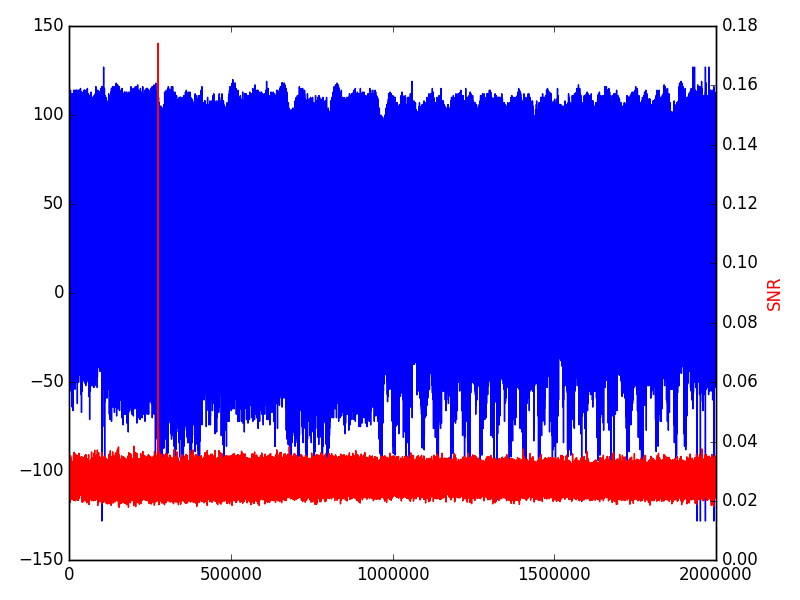
\includegraphics[scale=0.35]{figures/2Mpts/SNRK0_10ktraces.png}
	\caption{SNR targeting key byte 0 (in red), superposed to one leakage trace. SNR computed using $10.000$ traces.}
	\label{fig:SNR_K0}
\end{figure}

\subsection{Plaintext bytes}
Similarly, we perform a SNR targeting each plaintext byte as shown in Figure~\ref{fig:SNR_P0}. 
The results evidence three leakage points. The first leakage is explained by the loading of the plaintext in the target.
The second leakage is explained by the loading of the plaintext in the context (\texttt{Load\_data} function).
The third leakage is explained by the masking of the plaintext (\texttt{Map\_in\_G} function).

\begin{figure}[H]
	\centering 
	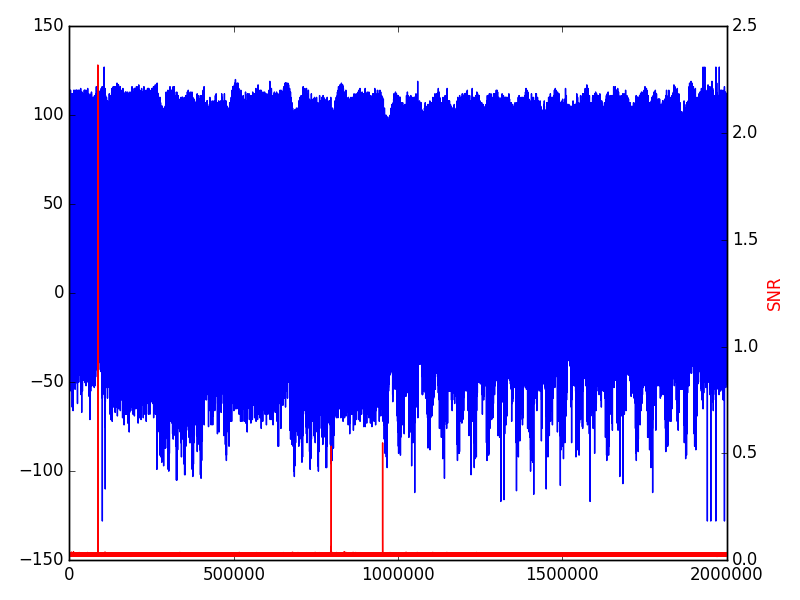
\includegraphics[scale=0.35]{figures/2Mpts/SNRP0_10ktraces.png}
	\caption{SNR targeting plaintext byte 0 (in red), superposed to one leakage trace. SNR computed using $10.000$ traces.}
	\label{fig:SNR_P0}
\end{figure}

\subsection{Ciphertext bytes}
Similarly, we perform a SNR targeting ciphertext bytes as shown in Figure~\ref{fig:SNR_C0}.
Leakages appear during the unmasking operation (\texttt{Multiplicative\_unmasking} function) and the serial writing of the bytes: when the ciphertext is loaded in the output variable.  %Note that the leakages occuring due to the serial writing do not appear for bytes 7 and plus, because of the limited trace size.

\begin{figure}[H]
	\centering 
	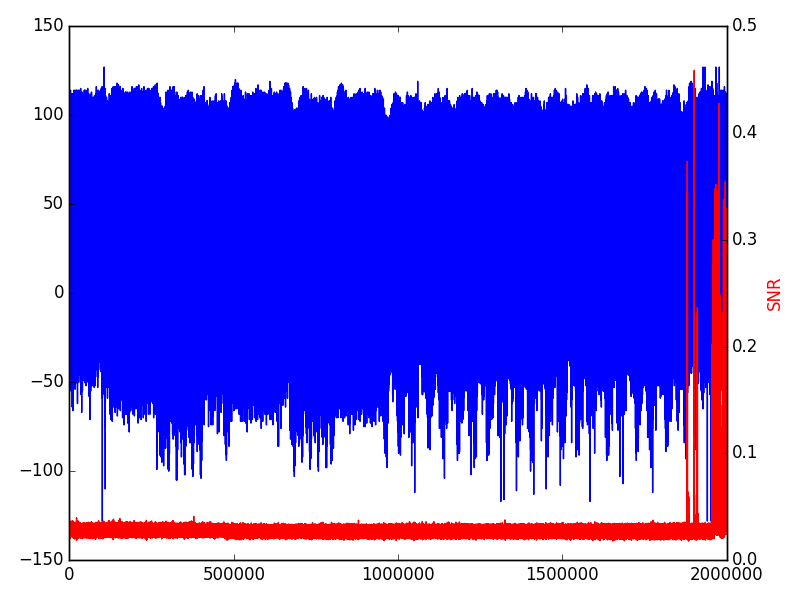
\includegraphics[scale=0.35]{figures/2Mpts/SNRC0_10ktraces.png}
	\caption{SNR targeting ciphertext byte 0 (in red), superposed to one leakage trace. SNR computed using $10.000$ traces.}
	\label{fig:SNR_C0}
\end{figure}

\subsection{Mask bytes}
Similarly, we perform a SNR targeting each mask byte. We detail the results hereafter, depending on the usages of each mask in the implementation.

\subsubsection{State masks}
Bytes $\maes[0]$ to $\maes[15]$, $\rin$, $\rout$ and $\rmult$ are used for the masking of the state of the encryption. We characterize hereafter their leakages.
 
Figure~\ref{fig:SNR_M0} and Figure~\ref{fig:SNR_M1} illustrate the results when targeting bytes $\maes[0]$ and $\maes[1]$. 
These bytes are used for computing both the shuffling permutation used in the substitution layer of the AES, and the permutations used in the linear layer. 
They are also used as linear masks.
Leakages appear during the loading of the bytes (\texttt{Load\_random} function).
Then, leakages appear during the computation of the shuffling permutation of the substitution layer, \texttt{Compute\_permIndices\_Tables}, and the computation of the permutations in the linear layer (\texttt{Compute\_permIndices\_Tables\_MC} functions).
Another leakage peak appears when the masks are loaded just before the encryption (\texttt{Load\_data} function), and a smaller peak appears when the state is masked (\texttt{Xor\_states} function).
Finally, we observe nine peaks corresponding to the 9 \texttt{MixColumns} operations.

\begin{figure}[H]
	\centering 
	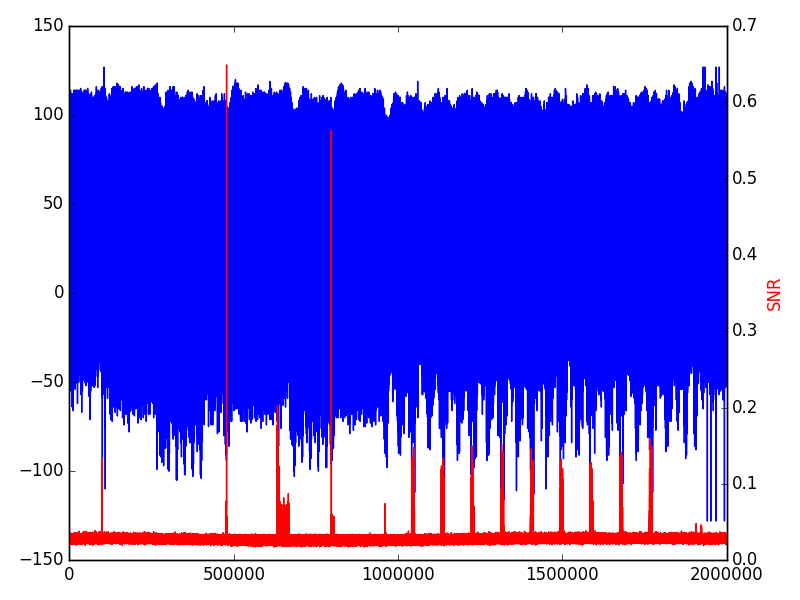
\includegraphics[scale=0.35]{figures/2Mpts/SNR_M0_10ktraces.png}
	\caption{SNR targeting mask byte $\maes[0]$ (in red), superposed to one leakage trace. SNR computed using $10.000$ traces.}
	\label{fig:SNR_M0}
	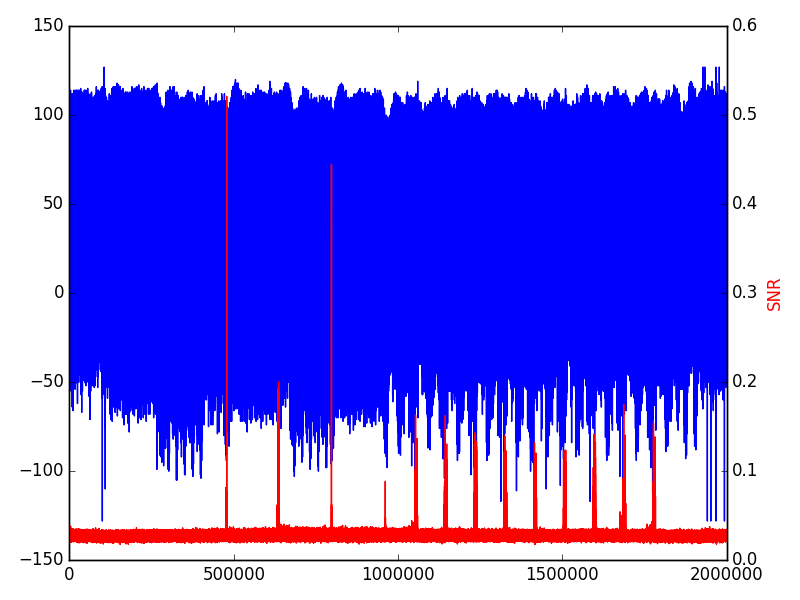
\includegraphics[scale=0.35]{figures/2Mpts/SNR_M1_10ktraces.png}
	\caption{SNR targeting mask byte $\maes[1]$ (in red), superposed to one leakage trace. SNR computed using $10.000$ traces.}
	\label{fig:SNR_M1}
\end{figure}

Figures~\ref{fig:SNR_M2} and~\ref{fig:SNR_M3} illustrate the results when targeting bytes $\maes[2]$ and $\maes[3]$. 
These bytes are used for computing the shuffling permutation used in the substitution layer, and as linear masks.
The leakages are similar to those of bytes $\maes[0]$ and $\maes[1]$, except that no leakage is observed during the \texttt{MixColumns} operations, nor during the computation of the permutations used in the linear layer.

\begin{figure}[H]
	\centering 
	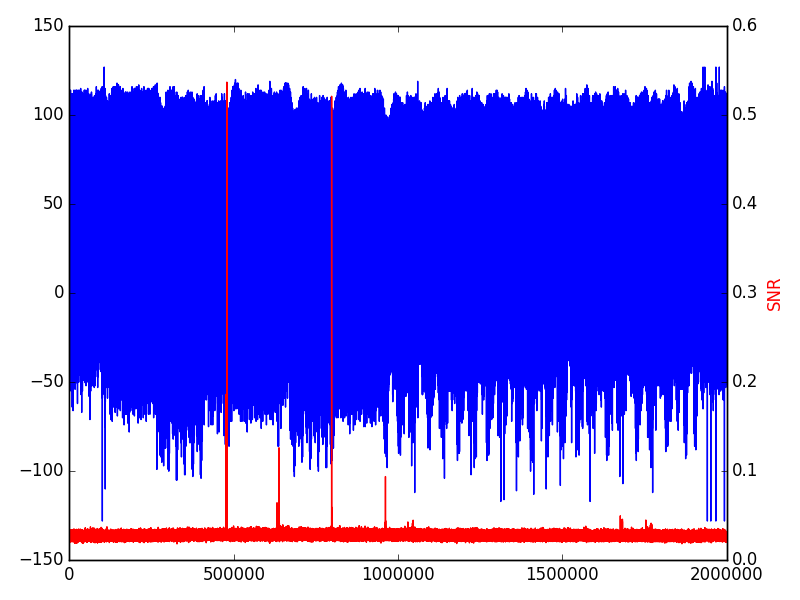
\includegraphics[scale=0.35]{figures/2Mpts/SNR_M2_10ktraces.png}
	\caption{SNR targeting mask byte $\maes[2]$ (in red), superposed to one leakage trace. SNR computed using $10.000$ traces.}
	\label{fig:SNR_M2}
	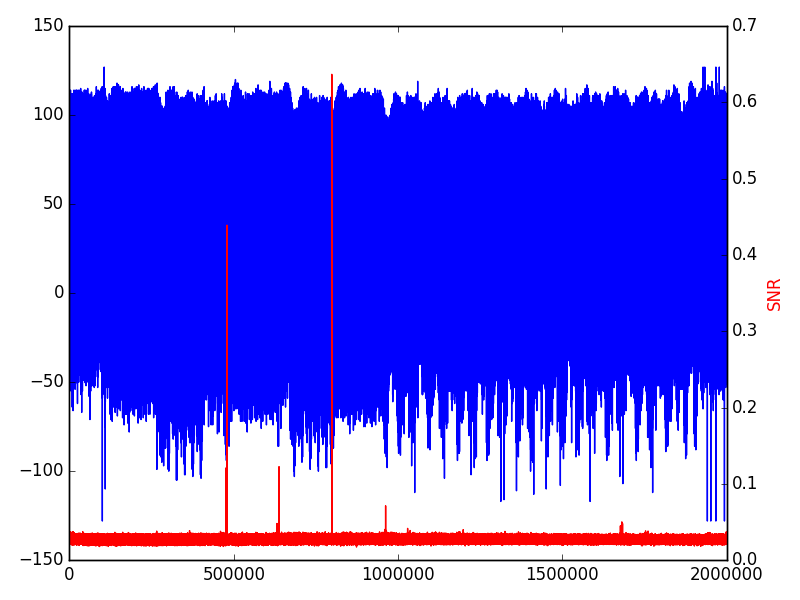
\includegraphics[scale=0.35]{figures/2Mpts/SNR_M3_10ktraces.png}
	\caption{SNR targeting mask byte $\maes[3]$ (in red), superposed to one leakage trace. SNR computed using $10.000$ traces.}
	\label{fig:SNR_M3}
\end{figure}

Figures~\ref{fig:SNR_M4} and \ref{fig:SNR_M15} illustrate the results when targeting bytes $\maes[4]$ and $\maes[15]$. These bytes are used as linear masks. Similar results are obtained for bytes $\maes[5]$ to $\maes[14]$.
The leakages are similar to the one obtained for previous bytes, but are now only observed for the loadings and masking of the state.
\begin{figure}[H]
	\centering 
	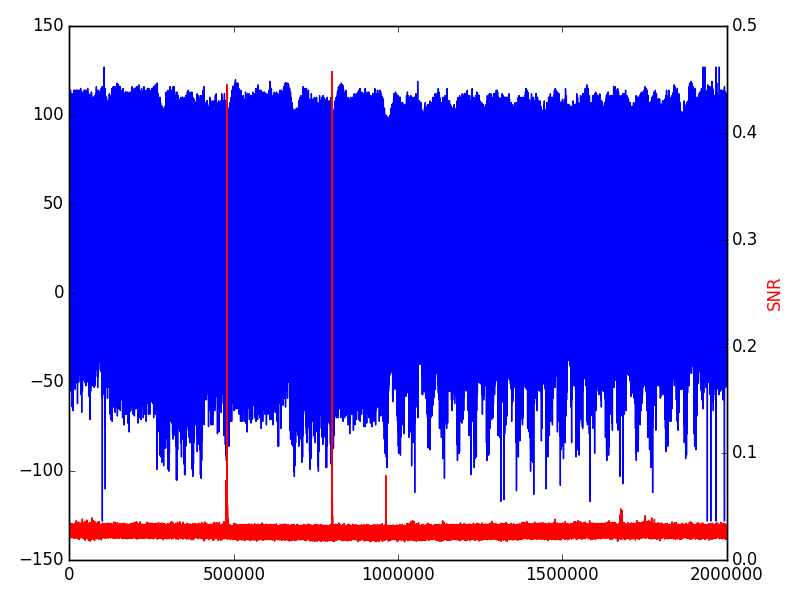
\includegraphics[scale=0.35]{figures/2Mpts/SNR_M4_10ktraces.png}
	\caption{SNR targeting mask byte $\maes[4]$ (in red), superposed to one leakage trace. SNR computed using $10.000$ traces.}
	\label{fig:SNR_M4}
	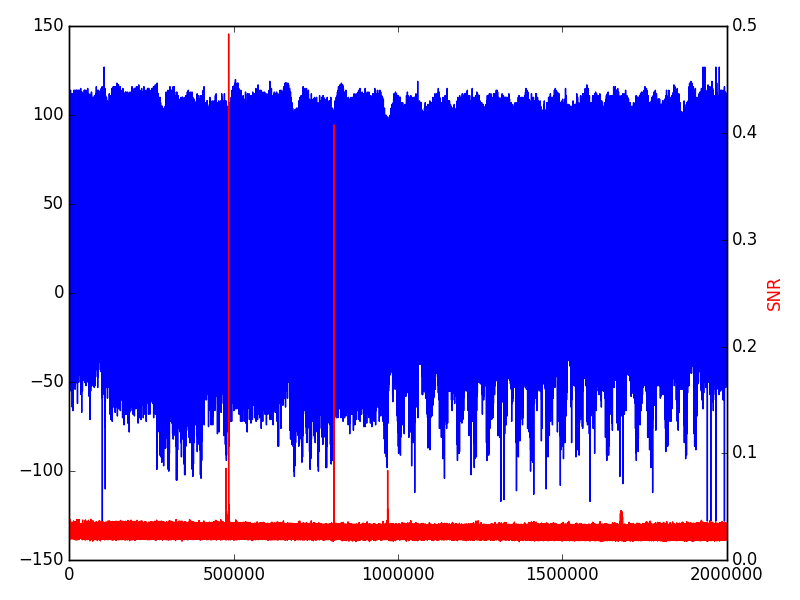
\includegraphics[scale=0.35]{figures/2Mpts/SNR_M15_10ktraces.png}
	\caption{SNR targeting mask byte $\maes[15]$ (in red), superposed to one leakage trace. SNR computed using $10.000$ traces.}
	\label{fig:SNR_M15}
\end{figure}

Figure~\ref{fig:SNR_rin} illustrates the results when targeting $\rin$. This byte is used as the input mask of the substition layer. 
Leakage first appears during the loading of the randoms (\texttt{Load\_data}).
Strong leakage can then be observed during the recomputation of the substitution table (\texttt{Compute\_Affine\_sboxMasked} function).
Finally 10 peaks appear during the substitution steps of each round of the AES.
\begin{figure}[H]
	\centering 
	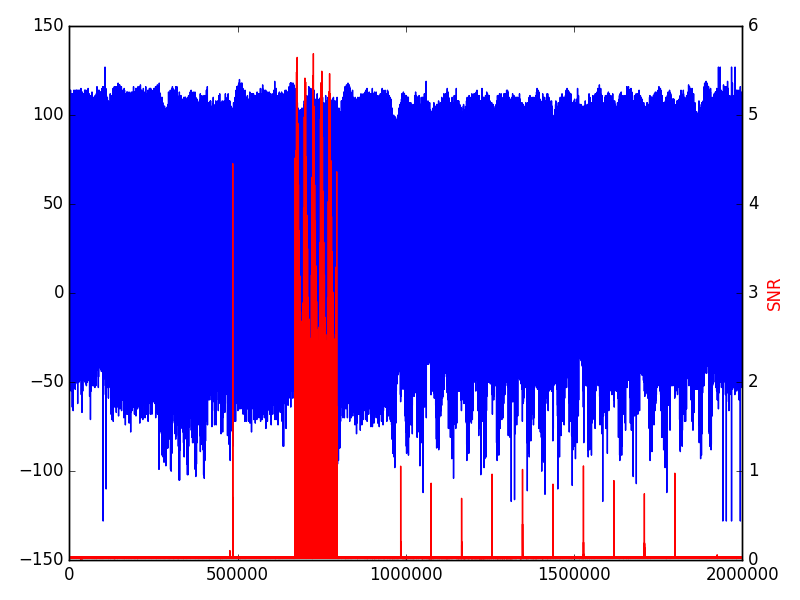
\includegraphics[scale=0.35]{figures/2Mpts/SNR_M16_10ktraces.png}
	\caption{SNR targeting mask byte $\rin $ (in red), superposed to one leakage trace. SNR computed using $10.000$ traces.}
	\label{fig:SNR_rin}
\end{figure}

Figure~\ref{fig:SNR_beta} illustrates the results when targeting $\rout$. This byte is used as the output mask of the subtitution layer. 
Leakages appear at similar time samples as for $\rin$.
\begin{figure}[H]
	\centering 
	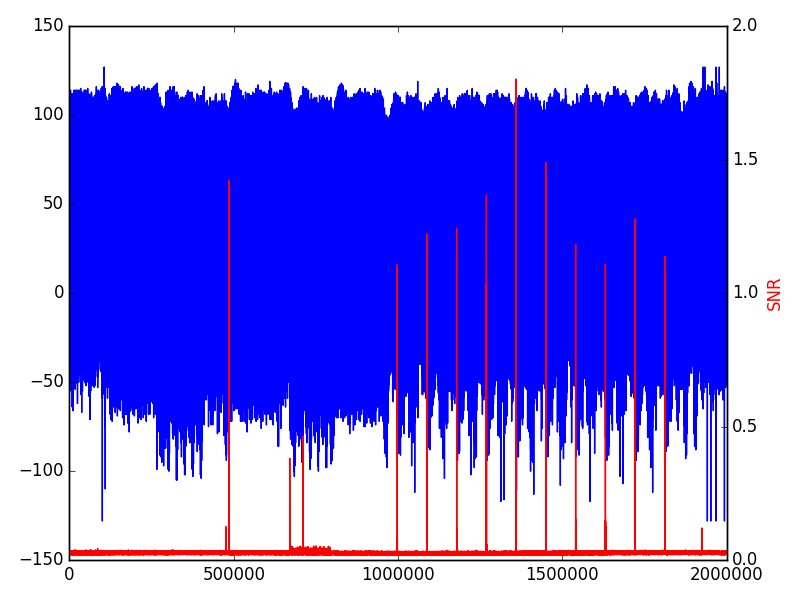
\includegraphics[scale=0.35]{figures/2Mpts/SNR_M17_10ktraces.png}
	\caption{SNR targeting mask byte $\rout$ (in red), superposed to one leakage trace. SNR computed using $10.000$ traces.}
	\label{fig:SNR_beta}
\end{figure}

Figure~\ref{fig:SNR_alpha} illustrates the results when targeting $\rmult$. This byte is used as the multiplicative mask of the substitution layer.
Leakage once again appear when the randoms are loaded (\texttt{Load\_data} function).
Leakage also appear during the computation of the multiplicative table (\texttt{Compute\_GTab} function), and during the computation of the substitution box (\texttt{Compute\_Affine\_sboxMasked} function).
\begin{figure}[H]
	\centering 
	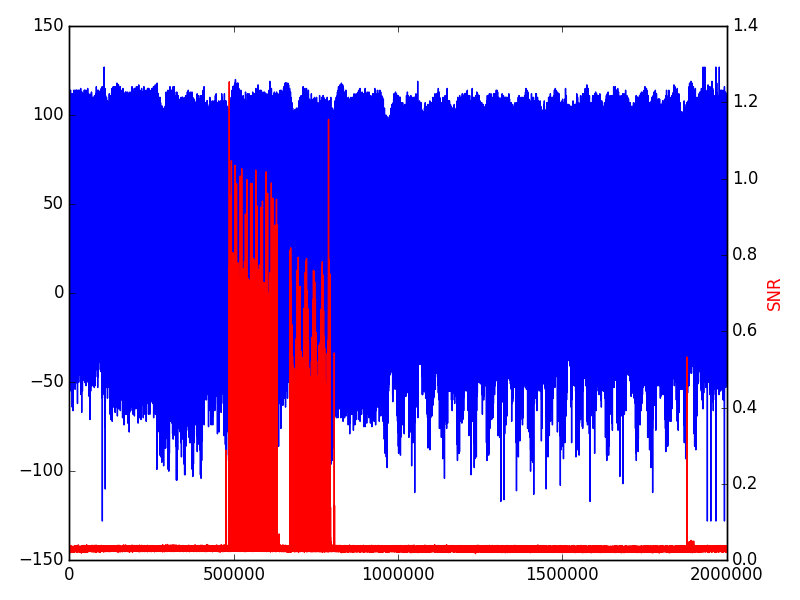
\includegraphics[scale=0.35]{figures/2Mpts/SNR_M18_10ktraces.png}
	\caption{SNR targeting mask byte $\rmult$ (in red), superposed to one leakage trace. SNR computed using $10.000$ traces.}
	\label{fig:SNR_alpha}
\end{figure}

\subsubsection{Key masks}
Bytes $\mkey[0]$ to $\mkey[15]$, $\rin'$, $\rout'$ and $\rmult'$ are used for the masking of the key. We characterize hereafter their leakages.
Figure~\ref{fig:SNR_M19} illustrates the results when targeting byte $\mkey[0]$. 
These bytes are used for computing the shuffling permutation used in the key expansion.
They are also used as linear masks.

Observed peaks correspond to the loading of the random in the target, loading of the masks (\texttt{Load\_random\_key} function), masking of the key (\texttt{Load\_masterKey}),
and the key expansion (\texttt{KeyExpansion\_masked} function), due to the involvment of the mask byte in the computation of the shuffling permutation\\ (\texttt{Compute\_permIndices\_Tables\_MC} function).

\begin{figure}[H]
	\centering 
	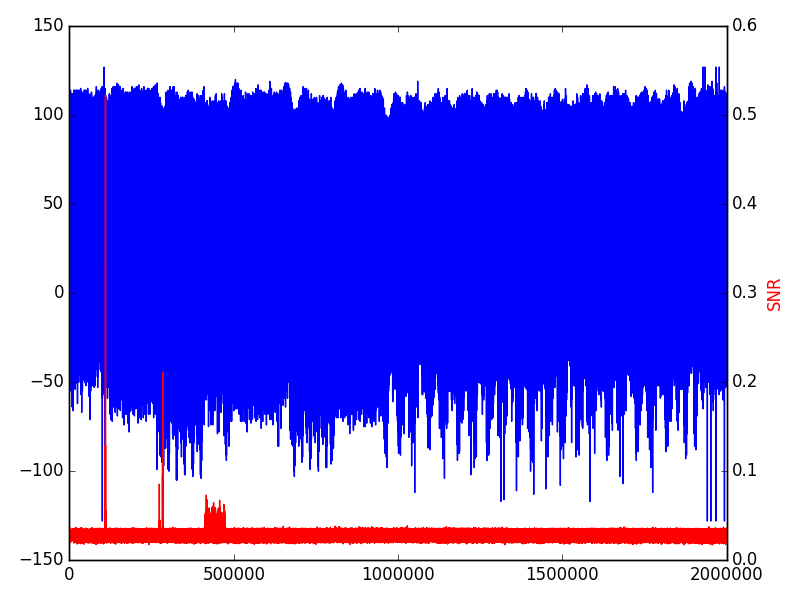
\includegraphics[scale=0.35]{figures/2Mpts/SNR_M19_10ktraces.png}
	\caption{SNR targeting mask byte $\mkey[0]$ (in red), superposed to one leakage trace. SNR computed using $10.000$ traces.}
	\label{fig:SNR_M19}
\end{figure}

Figures~\ref{fig:SNR_M20} and~\ref{fig:SNR_M21} illustrate the results when targeting bytes $\mkey[1]$ and $\mkey[2]$.  Similar results are observed when targeting bytes $\mkey[3]$ to $\mkey[15]$.
These bytes are not used for the computation of the shuffling permutation. However, they  serve as linear masks during the key expansion, and, as such, a small peak appears at the beginning of the \texttt{KeyExpansion\_masked} function.
The other peaks are similar to the ones appearing for byte $\mkey[0]$.

\begin{figure}[H]
	\centering 
	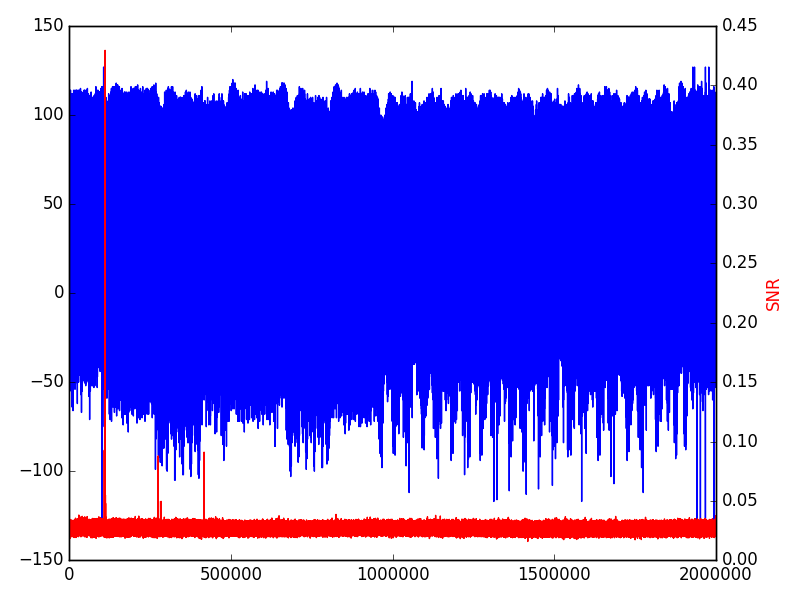
\includegraphics[scale=0.35]{figures/2Mpts/SNR_M20_10ktraces.png}
	\caption{SNR targeting mask byte $\mkey[1]$ (in red), superposed to one leakage trace. SNR computed using $10.000$ traces.}
	\label{fig:SNR_M20}
	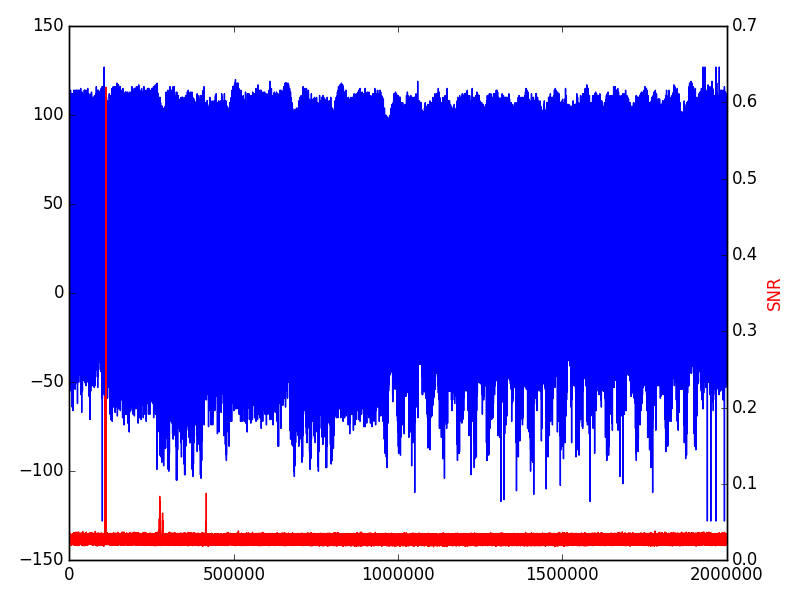
\includegraphics[scale=0.35]{figures/2Mpts/SNR_M21_10ktraces.png}
	\caption{SNR targeting mask byte $\mkey[2]$ (in red), superposed to one leakage trace. SNR computed using $10.000$ traces.}
	\label{fig:SNR_M21}
\end{figure}


Figure~\ref{fig:SNR_rin2} illustrates the results when targeting $\rin'$. This byte is used as the input mask of the substition layer.
Leakages appear at the same time samples as for bytes $\mkey[1]$ to $\mkey[15]$, and also during the recomputation of the Sbox and the key expansion.
\begin{figure}[H]
	\centering 
	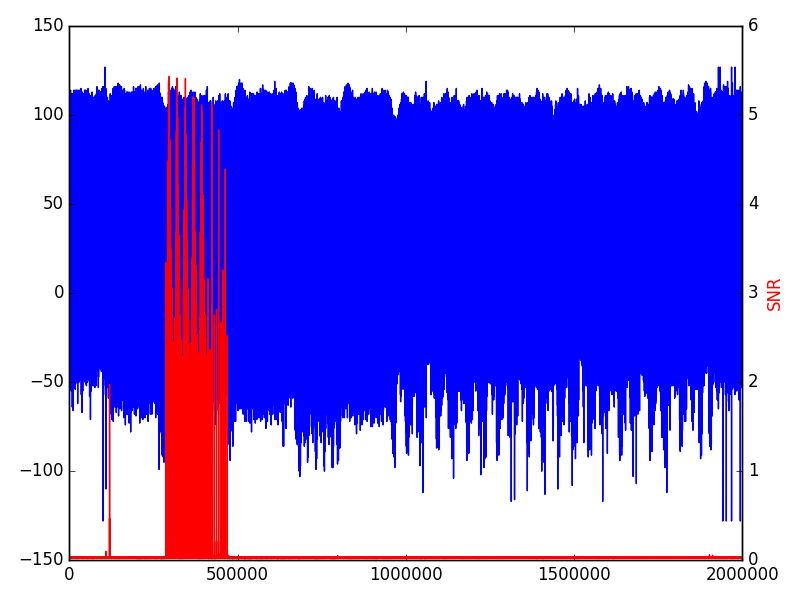
\includegraphics[scale=0.35]{figures/2Mpts/SNR_M35_10ktraces.png}
	\caption{SNR targeting mask byte $\rin'$ (in red), superposed to one leakage trace. SNR computed using $10.000$ traces.}
	\label{fig:SNR_rin2}
\end{figure}

Figure~\ref{fig:SNR_beta2} illustrates the results when targeting $\rout'$. This byte is used as the output mask of the subtitution layer. 
Leakages appear at the same time samples as for bytes $\mkey[1]$ to $\mkey[15]$, and also during the recomputation of the Sbox and the key expansion.
\begin{figure}[H]
	\centering 
	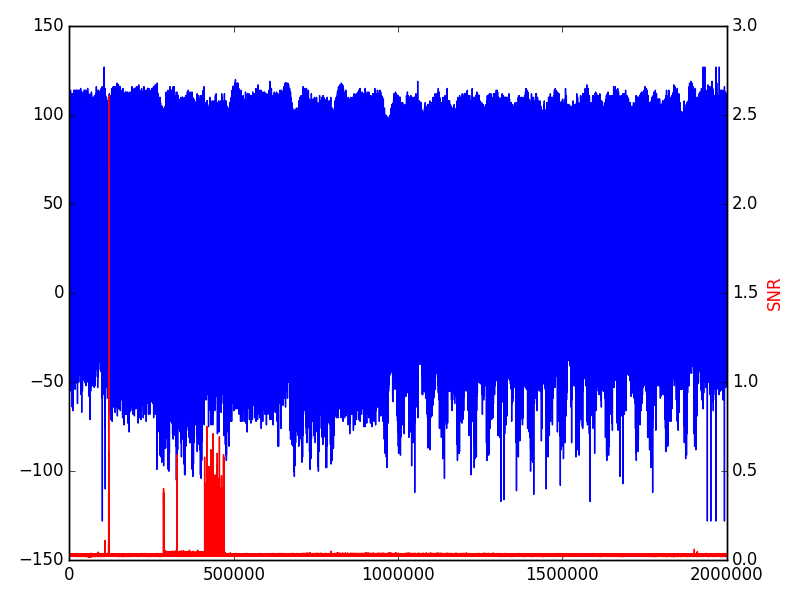
\includegraphics[scale=0.35]{figures/2Mpts/SNR_M36_10ktraces.png}
	\caption{SNR targeting mask byte $\rout'$ (in red), superposed to one leakage trace. SNR computed using $10.000$ traces.}
	\label{fig:SNR_beta2}
\end{figure}

Figure~\ref{fig:SNR_alpha2} illustrates the results when targeting byte $\rmult'$. This byte is used as the multiplicative mask of the substitution layer.
Leakages appear at the same time samples as the previous bytes, and also during the computation of the multiplication table \texttt{Gtab}.
Finally, a peak appears just before the encryption, when the value is loaded.
\begin{figure}[H]
	\centering 
	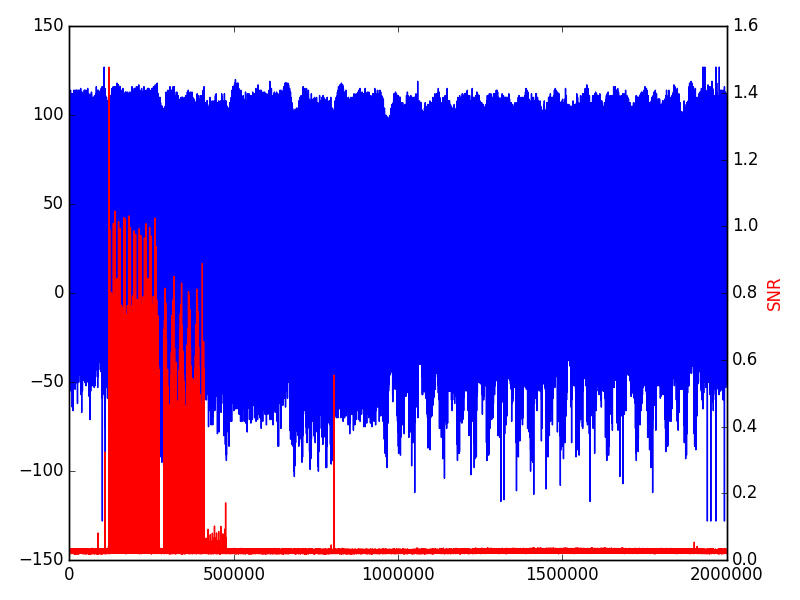
\includegraphics[scale=0.35]{figures/2Mpts/SNR_M37_10ktraces.png}
	\caption{SNR targeting mask byte $\rmult'$ (in red), superposed to one leakage trace. SNR computed using $10.000$ traces.}
	\label{fig:SNR_alpha2}
\end{figure}

\subsection{Sbox output bytes}
\subsubsection{Raw bytes}
Figure~\ref{fig:SNR_S0} illustrates the results when targeting a Sbox output byte without taking into account the output mask (ie. for each byte $i$, the value $S[\plain[i]\oplus \key[i]]$ is targeted) and there is no observable leakage.
\begin{figure}[H]
	\centering 
	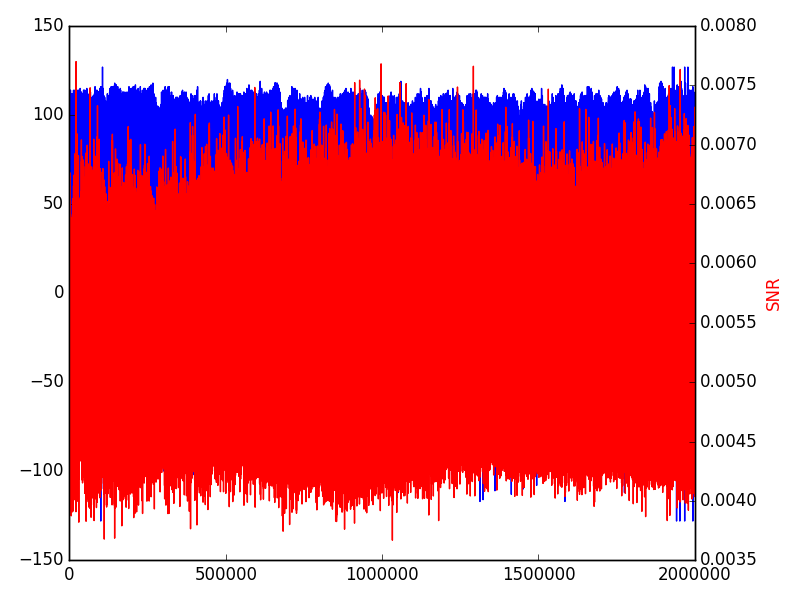
\includegraphics[scale=0.35]{figures/2Mpts/SNR_raw_S0_50ktraces.png}
	\caption{SNR targeting Sbox output byte 0 (in red), superposed to one leakage trace. SNR computed using $50.000$ traces.}
	\label{fig:SNR_S0}
\end{figure}

\subsubsection{Multiplied by mask} 
Figure~\ref{fig:SNR_aS0} illustrates the results when targeting a byte of the Sbox output, multiplied by the multiplicative mask, ie., for each byte $i$, the value $\rmult \times S[\plain[i]\oplus \key[i]]$ is targeted. No significant leakage is observed.
\begin{figure}[H]
	\centering 
	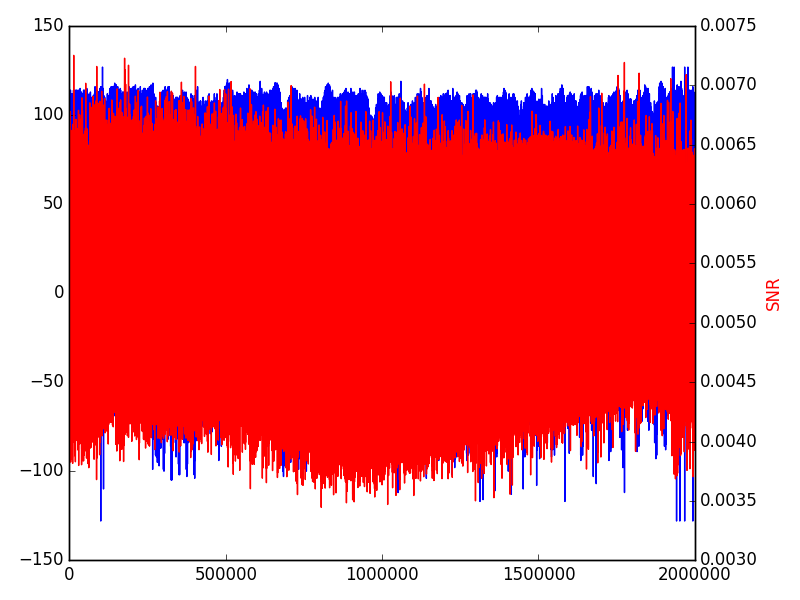
\includegraphics[scale=0.35]{figures/2Mpts/SNR_raw_aS0_50ktraces.png}
	\caption{SNR targeting the multiplicatively masked Sbox output byte 0 (in red), superposed to one leakage trace. SNR computed using $50.000$ traces.}
	\label{fig:SNR_aS0}
\end{figure}

\subsubsection{Affine masked}
Figure~\ref{fig:SNR_aS0+b} illustrates the results when targeting a byte of the Sbox output, affinely masked, ie., for each byte $i$, the value $\rmult \times S[P[i]\oplus K[i]] \oplus \rout$ is targeted. We remark that $50.000$ traces are not enough to highlight a leakage of this value.
This result is expected because of the shuffling countermeasure.
\begin{figure}[H]
	\centering 
	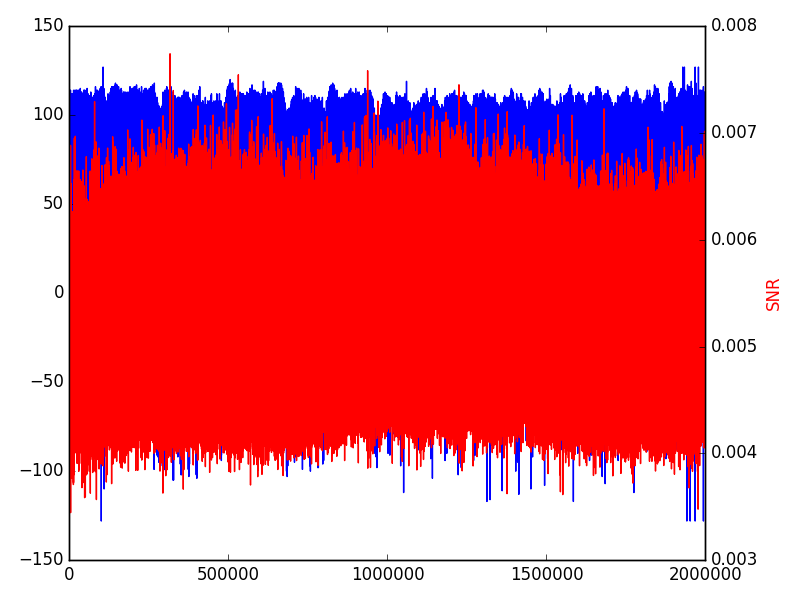
\includegraphics[scale=0.35]{figures/2Mpts/SNR_raw_aS+b0_50ktraces.png}
	\caption{SNR targeting the affinely masked Sbox output byte 0 (in red), superposed to one leakage trace. SNR computed using $50.000$ traces.}
	\label{fig:SNR_aS0+b}
\end{figure}


\subsection{Unshuffled output bytes}
\subsubsection{Raw bytes}
We use the knowledge of the mask bytes to inverse the shuffling $Sh$ performed during the substitution phase. For each index $i$, we target the value $S[\plain[Sh[i]]\oplus \key[Sh[i]]] $. No significant leakage can be observed. 
Figure~\ref{fig:SNR_unshuffledS0} illustrates the results.
\begin{figure}[H]
	\centering 
	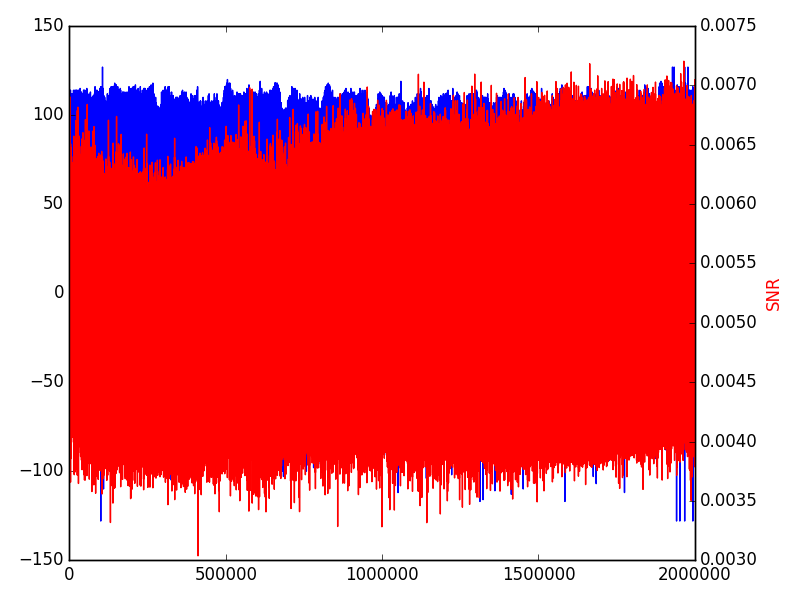
\includegraphics[scale=0.35]{figures/2Mpts/SNR_unshuffled_S0_50ktraces.png}
	\caption{SNR targeting the unshuffled Sbox output byte 0 (in red), superposed to one leakage trace. SNR computed using $50.000$ traces.}
	\label{fig:SNR_unshuffledS0}
\end{figure}

\subsubsection{Multiplicately masked}
We use the knowledge of the mask bytes to inverse the shuffling $Sh$ performed during the substitution phase. For each index $i$, we target the value $\rmult \times S[\plain[Sh(i)]\oplus \key[Sh(i)]]$. A small amount of leakage is present, at the time of the manipulation of $\rmult$. This is easily explained since the random variables $\rmult \times S[\plain[Sh(i)]\oplus \key[Sh(i)]]$ and $\rmult$ are not independent. 
Figure~\ref{fig:SNR_unshuffledaS0} illustrates the results.
\begin{figure}[H]
	\centering 
	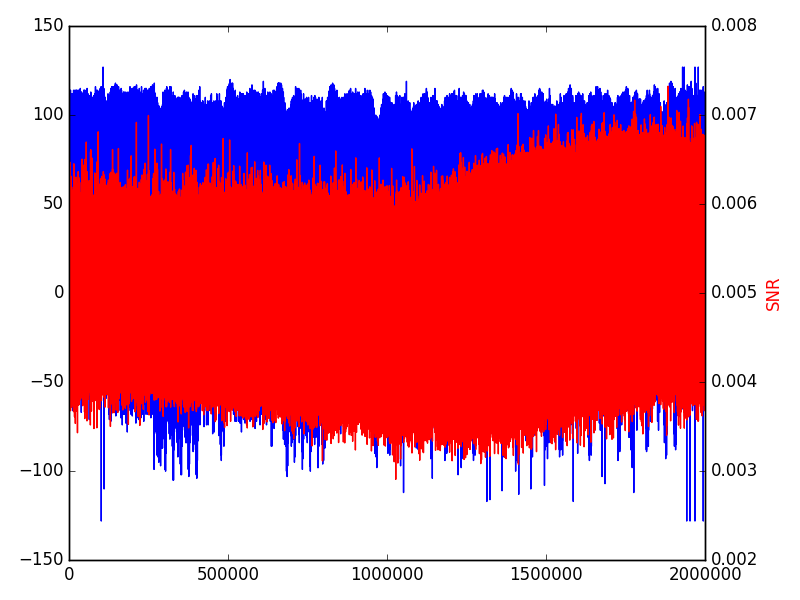
\includegraphics[scale=0.35]{figures/2Mpts/SNR_unshuffled_aS0_50ktraces.png}
	\caption{SNR targeting the unshuffled multiplicatively masked Sbox output byte 0 (in red), superposed to one leakage trace. SNR computed using $50.000$ traces.}
	\label{fig:SNR_unshuffledaS0}
\end{figure}

\subsubsection{Affinely masked}
We use the knowledge of the mask bytes to inverse the shuffling $Sh$ performed during the substitution phase. For each index $i$, we target the value $\rmult \times S[\plain[Sh(i)]\oplus \key[Sh(i)]] \oplus \rout$. A significant leakage is observed after the first substitution layer. %reprendre la notation pour le shuffle
Figure~\ref{fig:SNR_unshuffledaS0+b} illustrates the results.
\begin{figure}[H]
	\centering 
	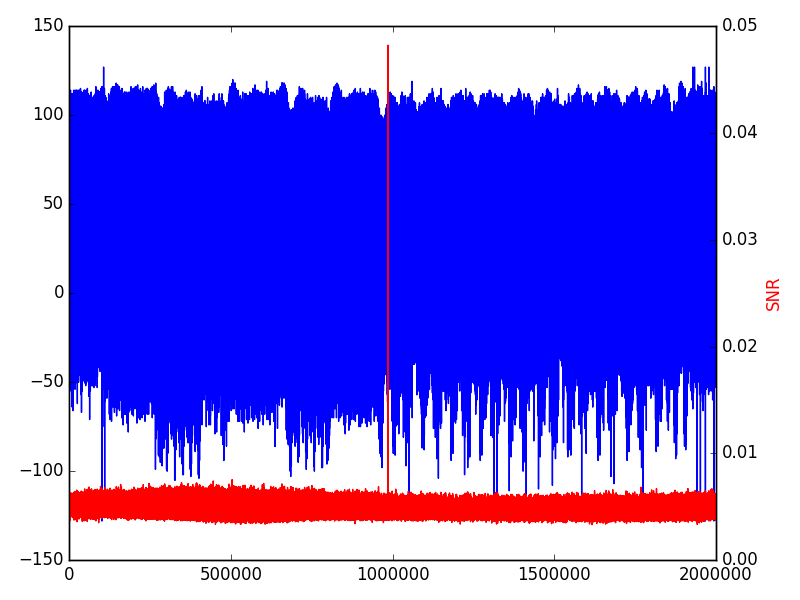
\includegraphics[scale=0.35]{figures/2Mpts/SNR_unshuffled_aS+b0_50ktraces.png}
	\caption{SNR targeting the unshuffled affinely masked Sbox output byte 0 (in red), superposed to one leakage trace. SNR computed using $50.000$ traces.}
	\label{fig:SNR_unshuffledaS0+b}
\end{figure}


